\chapter{F018-Compatible Direct Memory Access (DMA) Controller}
\label{cha:dmagic}

The MEGA65 includes an F018/F018A backward-compatible DMA controller.
Unlike in the C65, where the DMA controller exists as a separate
chip, it is part of the 45GS02 processor in the MEGA65.  However, as the
use of the DMA controller is a logically separate topic, it is documented
separately in this appendix.

The MEGA65's DMA controller provides several important improvements over the
F018/F018A DMAgic chips of the C65:

\begin{itemize}
\item{\bf Speed} The MEGA65 performs DMA operations at 40MHz, allowing filling 40MiB or copying 20MiB
  per second.  For example, it is possible to copy a complete 8KiB C64-style bitmap display in
  about 200 micro-seconds, equivalent to less than four raster lines!
 \item{\bf Large Memory Access} The MEGA65's DMA controller allows access to all 256MiB of address space.
\item{\bf Texture Copying Support} The MEGA65's DMA controller can do fractional address calculations
  to support hardware texture scaling, as well as address striding, to make it possible in principle
  to simultaneously scale-and-draw a texture from memory to the screen. This would be useful, should
  anyone be crazy enough to try to implement a Wolfenstein or Doom style-game on the MEGA65.
\item{\bf Transparency/Mask Value Support} The MEGA65's DMA controller can be told to ignore a special value
   when copying memory, leaving the destination memory contents unchanged. This allows masking of transparent
   regions when performing a DMA copy, which considerably simplifies blitting of graphics shapes.
\item{\bf Per-Job Option List} A number of options can be configured for each job in a chained list of DMA
  jobs, for example, selecting F018 or F018B mode, changing the transparency value, fractional address stepping
  or the source or destination memory region.

\item{\bf Background Audio DMA}
  The MEGA65 includes background audio DMA capabilities similar to the Amiga\texttrademark series of computers.
  Key differences are that the MEGA65 can use either 8 or 16-bit samples, supports very high sample rates
  up to approximately 1 MHz, has 256 volume settings per channel, and no inter-channel modulation.

\end{itemize}


\section{F018A/B DMA Jobs}

To execute a DMA job using the F018 series of DMA controllers, you must construct the list of DMA jobs in memory,
and then write the address of this list into the DMA address registers.  The DMA job will execute when you write to
the ADDRLSBTRIG register (\$D700).  For this reason you must write the MSB and bank number of the DMA list inti \$D701 and \$D702 first,
and the LSB only after having set these other two registers.  If you wish to execute multiple DMA jobs using the same
list structure in memory, you can simply write to ADDRLSBTRIG again after updating the list contents -- provided that
no other program has modified the contents of \$D701 or \$D702.  Note that BASIC 65 uses the DMA controller to
scroll the screen, so it is usually safest to always write to all three registers.

When ADDRLSBTRIG has been written to, the DMA job completes immediately.  Unlike on the C65, the DMA controller is part
of the processor of the MEGA65. This means that the processor stops trying to execute instructions {\em or fetching audio samples for DMA audio playback} until the DMA job
has completed.  It also means that, unlike on the C65, DMA jobs cannot be interrupted. If your program has sensitive timing
requirements, you may need to break larger DMA jobs into several smaller jobs.  This is somewhat mitigated by the high
speed of the MEGA65's DMA, which is able to fill memory at 40.5MiB per second and copy memory at 20.25MiB per second, compared
with circa 3.5 MiB and 1.7 MiB per second on a C65. This allows larger DMA jobs to be executed, without needing to worry about
the impact on real-time elements of a program. For example, it is possible to fill an 80 column 50 row text screen using the
MEGA65's DMA controller in just 200 microseconds.

\subsection{F018 DMA Job List Format}

The MEGA65's DMA controller supports the two different DMA job list formats used by the original F018 part that
was used in the earlier C65 prototypes (upto Revision 2B) and the F018B and later revisions used in the Revision 3 -- 5
C65 prototypes.  The main difference is the addition of a second command byte, as the following tables show:

It is important to know which style the DMA controller is expecting.  The MEGA65's Hypervisor sets the mode based on
the detected version of C65 ROM, if one is running. If it is an older one, then the F018 style is expected, otherwise
the newer F018B style is expected.  You can check which style has been selected by querying bit 0 of \$D703: If it is
a 1, then the newer F018B 12-byte list format is expected. If it is a 0, then the older F018 11-byte list format is expected.
The expected style can be set by writing to this register.

Unless you are writing software that must also run
on a C65 prototype, you should most probably use the MEGA65's Enhanced DMA Jobs, where the list format is explicitly specified
in the list itself.  As the Enhanced DMA Jobs are an extension of the F018/F018B DMA jobs, you should still read the following,
unless you are already familiar with the behaviour of the F018 DMA controller.

\subsubsection{F018 11-byte DMA List Structure}

\begin{tabular}{|c|l|}
  \hline
  Offset & Contents \\
  \hline
  \$00 & Command LSB \\
  \$01 & Count LSB \\
  \$02 & Count MSB \\
  \$03 & Source Address LSB  \\
  \$04 & Source Address MSB \\
  \$05 & Source Address BANK and FLAGS \\
  \$06 & Destination Address LSB  \\
  \$07 & Destination Address MSB \\
  \$08 & Destination Address BANK and FLAGS \\
  \$09 & Modulo LSB \\
  \$0a & Modulo MSB \\
  \hline
  \multicolumn{2}{l}{* The Command MSB is \$00 when using this list format.}

\end{tabular}

\subsubsection{F018B 12-byte DMA List Structure}

\begin{tabular}{|c|l|}
  \hline
  Offset & Contents \\
  \hline
  \$00 & Command LSB \\
  \$01 & Count LSB \\
  \$02 & Count MSB \\
  \$03 & Source Address LSB  \\
  \$04 & Source Address MSB \\
  \$05 & Source Address BANK and FLAGS \\
  \$06 & Destination Address LSB  \\
  \$07 & Destination Address MSB \\
  \$08 & Destination Address BANK and FLAGS \\
  \$09 & Command MSB \\
  \$0a & Modulo LSB / Mode \\
  \$0b & Modulo MSB / Mode \\
  \hline
\end{tabular}

The structure of the command word is as follows:

\begin{tabular}{|c|l|}
  \hline
  Bit(s) & Contents \\
  \hline
  0 -- 1 & DMA Operation Type \\
  2 & Chain (i.e., another DMA list follows) \\
  3 & Yield to interrupts \\
  4 & MINTERM -SA,-DA bit \\
  5 & MINTERM -SA,DA bit \\
  6 & MINTERM SA,-DA bit \\
  7 & MINTERM SA,DA bit \\
  8 -- 9 & Addressing mode of source \\
  10 -- 11 & Addressing mode of destination \\
  12 -- 15 & RESESRVED. Always set to 0's \\
  \hline
\end{tabular}

The command field take the following four values:

\begin{tabular}{|c|l|}
  \hline
  Value & Contents \\
  \hline
  \%00 (0) & Copy \\
  \%01 (1) & Mix (via MINTERMs) \\
  \%10 (2) & Swap \\
  \%11 (3) & Fill \\
  \hline
  \multicolumn{2}{l}{* Only Copy and Fill are implemented at the time of writing.}
\end{tabular}


The addressing mode fields take the following four values:

\begin{tabular}{|c|l|}
  \hline
  Value & Contents \\
  \%00 (0) & Linear (normal) addressing \\
  \%01 (1) & Modulo (rectangular) addressing \\
  \%10 (2) & Hold (constant address) \\
  \%11 (3) & XY MOD (bitmap rectangular) addressing \\
  \hline
  \multicolumn{2}{l}{* Only Linear, Modulo and Hold are implemented at the time of writing.}
\end{tabular}

The BANK and FLAGS field for the source address allow selection of addresses within a 1MB
address space. To access memory beyond the first 1MB, it is necessary to use an Enhanced DMA
Job with the appropriate option bytes to select the source and/or destination MB of memory.
The BLANKS and FLAGS field has the following structure:

\begin{tabular}{|c|l|}
  \hline
  Bit(s) & Contents \\
  0 -- 3 & Memory BANK within the selected MB \\
  4 & HOLD, i.e., do not change the address \\
  5 & MODULO, i.e., apply the MODULO field to wrap-around within a limited memory space \\
  6 & DIRECTION. If set, then the address is decremented instead of incremented. \\
  7 & I/O. If set, then IO registers are visible during the DMA controller at \$D000 -- \$DFFF. \\
  \hline
\end{tabular}

\subsubsection{Performing Simple DMA Operations}

For information on using the DMA controller from BASIC 65, refer to the \stw{DMA} BASIC command in \bookvref{BASIC 65 Commands!DMA}.

To use the DMA controller from assembly language, set up a data structure with the DMA list, and then
set \$D702 -- \$D700 to the address of the list. For example, to clear the screen in C65 mode by filling
it with spaces, the following routine could be used:

\begin{tcolorbox}[colback=black,coltext=white]
\verbatimfont{\codefont}
\begin{verbatim}
  LDA #$00       ; DMA list exists in BANK 0
  STA $D702
  LDA #>dmalist  ; Set MSB of DMA list address
  STA $D701
  LDA #<dmalist  ; Set LSB of DMA list address, and execute DMA
  STA $D700
  RTS

dmalist:
  .byte $03   ; Command low byte: FILL
  .word 2000  ; Count: 80x25 = 2000 bytes
  .word $0020 ; Fill with value $20
  .byte $00   ; Source bank (ignored with FILL operation)
  .word $0800 ; Destination address where screen lives
  .byte $00   ; Screen is in bank 0
  .byte $00   ; Command high byte
  .word $0000 ; Modulo (ignored due to selected commmand)
\end{verbatim}
\end{tcolorbox}

It is also possible to execute more than one DMA job at the same time, by setting the CHAIN
bit in the low-byte of the command word. For example to clear the screen as above, and
also clear the colour RAM for the screen, you could use something like:

\begin{tcolorbox}[colback=black,coltext=white]
\verbatimfont{\codefont}
\begin{verbatim}
  LDA #$00       ; DMA list exists in BANK 0
  STA $D702
  LDA #>dmalist  ; Set MSB of DMA list address
  STA $D701
  LDA #<dmalist  ; Set LSB of DMA list address, and execute DMA
  STA $D700
  RTS

dmalist:
  .byte $04   ; Command low byte: FILL + CHAIN
  .word 2000  ; Count: 80x25 = 2000 bytes
  .word $0020 ; Fill with value $20
  .byte $00   ; Source bank (ignored with FILL operation)
  .word $0800 ; Destination address where screen lives
  .byte $00   ; Screen is in bank 0
  .byte $00   ; Command high byte
  .word $0000 ; Modulo (ignored due to selected commmand)

  ; Second DMA job immediately follows the first
  .byte $03   ; Command low byte: FILL
  .word 2000  ; Count: 80x25 = 2000 bytes
  .word $0001 ; Fill with value $01 = white
  .byte $00   ; Source bank (ignored with FILL operation)
  .word $F800 ; Destination address where colour RAM lives
  .byte $01   ; colour RAM is in bank 1 ($1F800-$1FFFF)
  .byte $00   ; Command high byte
  .word $0000 ; Modulo (ignored due to selected commmand)
\end{verbatim}
\end{tcolorbox}

Copying memory is very similar to filling memory, except that the command
low byte must be modified, and the source address field must be correctly initialised.
For example, to copy the character set from where it lives in the ROM at \$2D000 -- \$2DFFF
to \$5000, you could use something like:

\begin{tcolorbox}[colback=black,coltext=white]
\verbatimfont{\codefont}
\begin{verbatim}
  LDA #$00       ; DMA list exists in BANK 0
  STA $D702
  LDA #>dmalist  ; Set MSB of DMA list address
  STA $D701
  LDA #<dmalist  ; Set LSB of DMA list address, and execute DMA
  STA $D700
  RTS

dmalist:
  .byte $00   ; Command low byte: COPY
  .word $1000 ; Count: 4KB = 4096
  .word $D000 ; Copy from $xD000
  .byte $02   ; Source bank = $02 for $2xxxx
  .word $5000 ; Destination address where screen lives
  .byte $00   ; Screen is in bank 0
  .byte $00   ; Command high byte
  .word $0000 ; Modulo (ignored due to selected commmand)
\end{verbatim}
\end{tcolorbox}

It is also possible to perform a DMA operation from BASIC 2 in C64
mode by POKEing the necessary values, after first making sure that
MEGA65 or C65 IO mode has been selected by writing the appropriate
values to \$D02F (53295). For example, to clear the screen in C64 BASIC 2
using the DMA controller, you could use something like:

\begin{tcolorbox}[colback=black,coltext=white]
\verbatimfont{\codefont}
\begin{verbatim}
10 rem enable mega65 I/O
20 poke53295,asc("g"):poke53295,asc("s")
30 rem dma list in data statements
40 data 3: rem command lsb = fill
50 data 232,3 : rem screen is 1000 bytes = 3*256+232
60 data 32,0: rem fill with space = 32
70 data 0: rem source bank (unused for fill)
80 data 0,4: rem screen address = 1024 = 4*256
90 data 0: rem screen lives in bank 0
100 data 0: rem command high byte
110 data 0,0: rem modulo (unused in this job)
120 rem put dma list at $c000 = 49152
130 fori=0to11:reada:poke49152+i,a:next
140 rem execute job
150 poke55042,0: rem dma list is in bank 0
160 poke55041,192: rem dma list is in $c0xx
170 poke55040,0: rem dma list is in $xx00, and execute
\end{verbatim}
\end{tcolorbox}


While this is rather cumbersome to do each time, if you wanted to clear
the screen again, all you would need to do would be to \stw{POKE 55040,0} again,
assuming that the DMA list and DMA controller registers had not been modified
since the previous time the DMA job had been run.

The HOLD, IO and other options can also be used to create interesting effects.
For example, to write a new value to the screen background colour very quickly,
you could copy a region of memory to \$D021, with the IO flag set to make the IO
register visible for writing in the DMA job, and the HOLD flag set, so that the
same address gets written to repeatedly. This will write to the background colour
at a rate of 20.5MHz, which is almost as fast as the video pixel clock (27MHz).
Thus we can change the colour almost every pixel.

With a little care, we can make this routine such that it takes exactly one raster-line
to run, and thus draw vertical raster bars, or to create a kind of frankenstein video mode
that uses a linear memory layout -- at the cost of consuming all of the processor's time
during the active part of the display.

The following example does this to draw vertical raster bars on the screen.
This program assumes that the MEGA65 is set to PAL.  For NTSC, the size of the DMA transfer
would need to be decreased a little.  The other thing to note with this program, is that
it uses MEGA65 Enhanced DMA Job option \$81 to set the destination mega-byte in memory to
\$FFxxxxx, and the bank is set to \$D, and the destination address to \$0021, to form the
complete address \$FFD0021.  This is the true location of the VIC-IV's border colour register.
The program is written using ACME-compatible syntax.

\begin{tcolorbox}[colback=black,coltext=white]
\verbatimfont{\codefont}
\begin{verbatim}
basicheader:
	;; 2020 SYS 2061
	!word $80a,2020
	!byte $9e,$32,$30,$36,$31,0,0,0

	;; Actual code begining at $080d = 2061
main:
	sei
	lda #$47        	; enable MEGA65 IO
	sta $D02f
	lda #$53
	sta $d02f
	lda #65 		; Set CPU speed to fast
	sta 0
	lda #0            	; disable screen to show only the border
	sta $d011

	lda $d012              	; Wait until start of the next raster
raster_sync:	  		; before beginning loop for horizontal alignment
	cmp $d012
	beq raster_sync

	;; The following loop takes exactly one raster line at 40.5MHz in PAL
loop:
	jsr triggerdma
	jmp loop

triggerdma:
	lda #0			; make sure F018 list format
	sta $d703

	lda #0     		; dma list bank
	sta $d702
	lda #>rasterdmalist
	sta $d701
	lda #<rasterdmalist
	sta $d705
	rts
\end{verbatim}
\end{tcolorbox}

\begin{tcolorbox}[colback=black,coltext=white]
\verbatimfont{\codefont}
\begin{verbatim}
rasterdmalist:
	!byte $81,$ff,$00
	!byte $00 		; COPY
	!word 619 		; DMA transfer is 619 bytes long
	!word rastercolours	; source address
	!byte $00               ; source bank
	!word $0020		; destination address
	!byte $1d               ; destination bank + HOLD
	;; unused modulo field
	!word $0000
\end{verbatim}
\end{tcolorbox}

\begin{tcolorbox}[colback=black,coltext=white]
\verbatimfont{\codefont}
\begin{verbatim}
rastercolours:
	!byte 0,0,0,0,0,0,0,0,0,0,0,0,0,0
	!byte 0,0,0,11,11,11,12,12,12,15,15,15,1,1,1,15,15,15,12,12,12,11,11,11,0,0,0
	!byte 0,0,0,6,6,6,4,4,4,14,14,14,3,3,3,1,1,1,3,3,3,14,14,14,4,4,4,6,6,6,0,0,0
	!byte 0,0,0,11,11,11,12,12,12,15,15,15,1,1,1,15,15,15,12,12,12,11,11,11,0,0,0
	!byte 0,0,0,6,6,6,4,4,4,14,14,14,3,3,3,1,1,1,3,3,3,14,14,14,4,4,4,6,6,6,0,0,0
	!byte 0,0,0,11,11,11,12,12,12,15,15,15,1,1,1,15,15,15,12,12,12,11,11,11,0,0,0
	!byte 0,0,0,6,6,6,4,4,4,14,14,14,3,3,3,1,1,1,3,3,3,14,14,14,4,4,4,6,6,6,0,0,0
	!byte 0,0,0,11,11,11,12,12,12,15,15,15,1,1,1,15,15,15,12,12,12,11,11,11,0,0,0
	!byte 0,0,0,6,6,6,4,4,4,14,14,14,3,3,3,1,1,1,3,3,3,14,14,14,4,4,4,6,6,6,0,0,0
	!byte 0,0,0,11,11,11,12,12,12,15,15,15,1,1,1,15,15,15,12,12,12,11,11,11,0,0,0
	!byte 0,0,0,6,6,6,4,4,4,14,14,14,3,3,3,1,1,1,3,3,3,14,14,14,4,4,4,6,6,6,0,0,0
	!byte 0,0,0,11,11,11,12,12,12,15,15,15,1,1,1,15,15,15,12,12,12,11,11,11,0,0,0
	!byte 0,0,0,6,6,6,4,4,4,14,14,14,3,3,3,1,1,1,3,3,3,14,14,14,4,4,4,6,6,6,0,0,0
	!byte 0,0,0,11,11,11,12,12,12,15,15,15,1,1,1,15,15,15,12,12,12,11,11,11,0,0,0
	!byte 0,0,0,6,6,6,4,4,4,14,14,14,3,3,3,1,1,1,3,3,3,14,14,14,4,4,4,6,6,6,0,0,0
	!byte 0,0,0,11,11,11,12,12,12,15,15,15,1,1,1,15,15,15,12,12,12,11,11,11,0,0,0
	!byte 0,0,0,6,6,6,4,4,4,14,14,14,3,3,3,1,1,1,3,3,3,14,14,14,4,4,4,6,6,6,0,0,0
	!byte 0,0,0,11,11,11,12,12,12,15,15,15,1,1,1,15,15,15,12,12,12,11,11,11,0,0,0
	!byte 0,0,0,6,6,6,4,4,4,14,14,14,3,3,3,1,1,1,3,3,3,14,14,14,4,4,4,6,6,6,0,0,0
\end{verbatim}
\end{tcolorbox}

\section{MEGA65 Enhanced DMA Jobs}

The MEGA65's implementation of the DMAgic supports significantly
enhanced DMA jobs.  An enhanced DMA job is indicated by writing the
low-byte of the DMA list address to \$D705 instead of to \$D700.  The
MEGA65 will then look for one or more {\em job option tokens} at the
start of the DMA list.  Those tokens will be interpretted, before
executing the DMA job which immediately follows the {\em end of job
  options} token (\$00).

Job option tokens that take an argument have the
most-significant bit set, and always take a 1 byte option.  Job option
tokens that take no argument have the most-significant-bit clear.
Unsupported job option tokens are simply ignored.
This allows for future revisions of the DMAgic to add support for
additional options, without breaking backward compatibility.

These options are also used to achieve advanced features, such as hardware
texture scaling at up to 20Mpixels per second, and hardware line drawing
at up to 40Mpixels per second. These advanced functions are implemented
by allowing complex calculations to be made to the source and/or destination
address of DMA jobs as they execute.

The list of valid job option tokens is:

\index{Line Drawing}
\index{Line Drawing!DMA Option Bytes}
\begin{tabular}{|c|p{10cm}|}
  \hline
  \$00 & End of job option list \\
  \$06 & Disable use of transparent value \\
  \$07 & Enable use of transparent value \\
  \$0A & Use 11-byte F011A DMA list format \\
  \$0B & Use 12-byte F011B DMA list format \\
  \$53 & Enable `Shallan Spiral' Mode \\
  \$80 & Source address bits 20 -- 27 \\
  \$81 & Destination address bits 20 -- 27 \\
  \$82 & Source skip rate (256\textsuperscript{ths} of bytes) \\
  \$83 & Source skip rate (whole bytes) \\
  \$84 & Destination skip rate (256\textsuperscript{ths} of bytes) \\
  \$85 & Destination skip rate (whole bytes) \\
  \$86 & Transparent value (bytes with matching value are not written) \\
  \$87 & Set X column bytes (LSB) for line drawing destination address \\
  \$88 & Set X column bytes (MSB) for line drawing destination address \\
  \$89 & Set Y row bytes (LSB) for line drawing destination address \\
  \$8A & Set Y row bytes (MSB) for line drawing destination address \\
  \$8B & Slope (LSB) for line drawing destination address \\
  \$8C & Slope (MSB) for line drawing destination address \\
  \$8D & Slope accumulator initial fraction (LSB) for line drawing destination address \\
  \$8E & Slope accumulator initial fraction (MSB) for line drawing destination address \\
  \$8F & Line Drawing Mode enable and options for destination address (set in argument byte): Bit 7 = enable line mode, Bit 6 = select X or Y direction, Bit 5 = slope is negative. \\
  \$97 & Set X column bytes (LSB) for line drawing source address \\
  \$98 & Set X column bytes (MSB) for line drawing source address \\
  \$99 & Set Y row bytes (LSB) for line drawing source address \\
  \$9A & Set Y row bytes (MSB) for line drawing source address \\
  \$9B & Slope (LSB) for line drawing source address \\
  \$9C & Slope (MSB) for line drawing source address \\
  \$9D & Slope accumulator initial fraction (LSB) for line drawing source address \\
  \$9E & Slope accumulator initial fraction (MSB) for line drawing source address \\
  \$9F & Line Drawing Mode enable and options for source address (set in argument byte): Bit 7 = enable line mode, Bit 6 = select X or Y direction, Bit 5 = slope is negative. \\
  
  \hline
\end{tabular}

\section{Texture Scaling and Line Drawing}
\index{Texture Scaling}

The DMAgic supports an advanced internal address calculator that allows it to draw scaled textures and draw
lines with arbitrary slopes on VIC-IV FCM video displays.

For texture scaling, the FCM screen must be arranged
vertically, as shown below:

\begin{center}
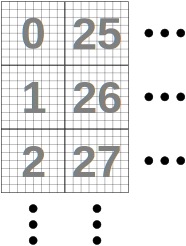
\includegraphics[width=0.7\textwidth]{images/illustrations/char-tile-grid-vertical-numbered}
\end{center}

By lining the characters into vertical columns like this, advancing vertically by one pixel adds a constant 8 bytes each time, as shown below:

\begin{center}
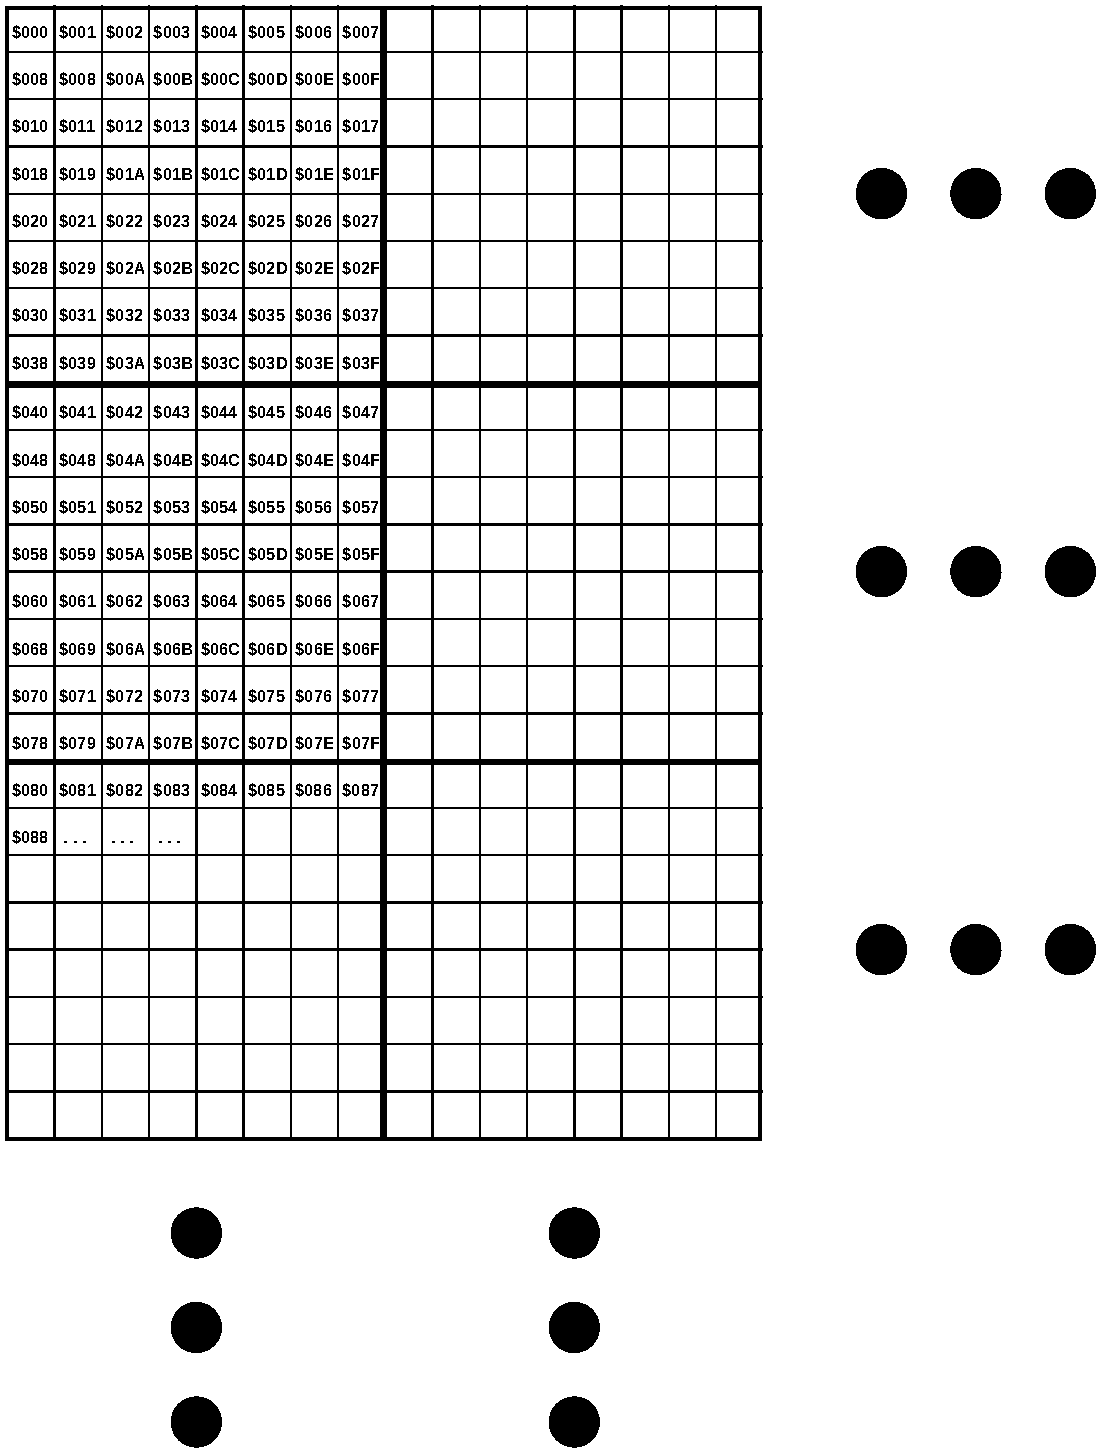
\includegraphics[width=0.7\textwidth]{images/illustrations/char-tile-grid-vertical-addressed}
\end{center}


The source and destination
skip rates also allow setting the scaling factors.  A skip rate of \$0100 this corresponds to stepping \$01.00 pixels.
To use the vertically stacked FCM layout as the target for copying vertical lines of textrures, then the destination
skip rate should be \$0800, i.e., 8.0 bytes per pixel.  This would copy a vertical line of texture data without scaling.
By setting the source stepping to < \$0100 will cause some pixels to be repeated, effectively zooming the texture in,
while setting the source stepping to > \$0100 will cause some pixels to be skipped, effectively zooming the texture out.
The destination stepping does not ordinary need to be adjusted.  Note that the texture data must be stored with each
vertical stripe stored contiguously, so that this mode can be used.

For line drawing, the DMA controller needs to know the screen layout, specifically, what number must be added to the
address of a rightmost pixel in one column of FCM characters in order to calculate the address of the pixel appearing
immediately to its right. Similarly, it must also know how much must be added to the address of a bottom most pixel in
one row of FCM characters in order to calculate the address of the pixel appearing immediately below it.  This allows
for flexible screen layout options, and arbitrary screen sizes.  You must then also specify the slope of the line, and
whether the line has the X or Y as its major axis, and whether the slope is positive or negative.

The file {\tt test\_290.c}
in the \url{https://github.com/mega65/mega65-tools} repository provides an example of using these facilities to
implement hardware accelerated line drawing. This is {\em very} fast, as it draws lines at the full DMA fill speed,
i.e., approximately 40,500,000 pixels per second.

\section{Audio DMA}
\index{Digital Audio}
\index{DMA Audio}
\index{Amiga(tm) style audio}
\index{MOD-file style audio}
The MEGA65 includes four channels of DMA-driven audio playback that can be used in place of the direct digital
audio registers at \$D6F8-\$D6FB.  That is, you must select which of these two sources to feed to the audio
cross-bar mixer.  This is selected via the AUDEN signal (\$D711 bit 7), which simultaneously enables the audio DMA
function in the processor, as well as instructing the audio cross-bar mixer to use the audio from this instead
of the \$D6F8-\$D6FB digital audio registers. If you wish to have no
other audio than the audio DMA channels, the audio cross-bar mixer can
be bypassed, and the DMA audio played at full volume by setting the
NOMIX signal (\$D711 bit 4).  In that mode no audio from the SIDs, FM,
microphones or other sources will be available.
All other bits in
\$D711 should ordinarily be left clear, i.e., write \$80 to \$D711 to
enable audio DMA.

Two channels form the left digital audio channel, and the other two
channels form the right digital audio channel. It is these left and
right channels that are then fed into the MEGA65's audio cross-bar
mixer.

As the DMA controller is part of the processor of the MEGA65, and the MEGA65 does not have reserved bus slots
  for multi-media operations, the MEGA65 uses idle CPU cycles to perform background DMA. This requires that the
  MEGA65 CPU be set to the ``full speed'' mode, i.e., approximately 40MHz.  In this mode, there is a wait-state
  whenever reading an operand from memory.  Thus each instruction that loads a byte from memory will create one
  implicit audio DMA slot.  This is rarely a problem in practice, except if the processor idles in a very tight
  loop.  To ensure that audio continues to play in the background, such loops should include a read instruction,
  such as:

\begin{screenoutput}
loop:   LDA $1234   // Ensure loop has at least one idle cycle for
                    // audio DMA
        JMP loop
\end{screenoutput}

Each of the four DMA channels is configured using a block of 16
registers at \$D720, \$D730, \$D740 and \$D750, respectively.
We will explain the registers for the first channel, channel 0, at
\$D720 -- \$D72F.

\subsection{Sample Address Management}

To play an audio sample you must first supply the start address of the
sample. This is a 24-bit address, and must be in the main chip memory
of the MEGA65. This is done by writing the address into \$D72A --
\$D72C.  This is the address of the first sample value that will be played.
You must then provide the end address of the sample in \$D727 --
\$D728.  But note that this is is only 16 bits. This is because the
MEGA65 compares only the bottom 16 bits of the address when checking
if it has reached the end of a sample.  In practice, this means that
samples cannot be more than 64KB in size.  If the sample contains a
section that should be repeated, then the start address of the
repeating part should be loaded into \$D721 -- \$D723, and the CH0LOOP
bit should be set (\$D720 bit 6).

You can determine the current sample address at any time by reading
the registers at \$D72A -- \$D72C. But beware: These registers are not
latched, so it is possible that the values may be updated as you read
the registers, unless you stop the channel first by clearing the CH0EN
signal.

\subsection{Sample Playback frequency and Volume}

The MEGA65 controls the playback rate of audio DMA samples by using a
24-bit counter.  Whenever the 24-bit counter overflows, the next
sample is requested. Sample speed control is achieved by setting the
value added to this counter each CPU cycle.  Thus a value of
\$FFFFFF would result in a sample rate of almost 40.5 MHz.  In
practice, sample rates above a few megahertz are not possible, because
there are insufficient idle CPU cycles, and distorted audio will
result.  Even below this, care must be taken to ensure that idle
cycles come sufficiently often and dispersed throughout the
processor's instruction stream to prevent distortion.  At typical
sample rates below 16KHz and using 8-bit samples these effects are
typically negligible for normal instruction streams, and so no special
action is normally required for typical audio playback.

At the other end of the scale, sample rates as low as 40.5MHz/$2^{24}$
= 2.4 samples per second are possible.  This is sufficiently low
enough for even the most demanding infra-sound applications.

Volume is controlled by setting \$D729.  Maximum volume is obtained
with the value \$FF, while a value of \$00 will effectively mute the
channel.  The first two audio channels are normally allocated to the
left, and the second two to the right.  However, the MEGA65 includes
separate volume controls for the opposite channels. For example, to
play audio DMA channel 0 at full volume on both left and right sides
of the audio output, set both \$D729 and \$D71C to \$FF.  This allows
panning of the four audio DMA channels.

Both the frequency and volume can be freely adjusted while a sample is playing
to produce various effects.

\subsection{Pure Sine Wave}

Where it is necessary to produce a stable sine wave, especially at
higher frequencies,
there is a special mode to support this. By setting the CH0SINE
signal, the audio channel will play a 32-byte 16-bit sine wave
pattern.  The sample addresses still need to be set, as though the
sine wave table were located in the bottom 64 bytes of memory, as the
normal address generation logic is used in this mode. However, no
audio DMA fetches are performed when a channel is in this mode, thus
avoiding all sources of distortion due to irregular spacing of idle
cycles in the processor's instruction stream.

This can be used to produce sine waves in both the audible range, as
well as well into the ultrasonic range, at frequencies exceeding
60,000Hz, provided that the MEGA65 is connected to an appropriately
speaker arrangement.

\subsection{Sample playback control}

To begin a channel playing a sample, set the CH0EN signal (\$D720 bit
7). The sample will play until its completion, unless the CH0LOOP
signal has also been set. When a sample completes playing, the CH0STP
flag will be set.  The audio DMA subsystem cannot presently generate
interrupts.

Unlike on the Amiga\texttrademark, the MEGA65 audio DMA system supports both
8 and 16-bit samples.  It also supports packed 4-bit samples, playing
either the lower or upper nybl of each sample byte.  This allows two
separate samples to occupy the same byte, thus effectively halving the
amount of space required to store two equal length samples.

\section{F018 ``DMAgic'' DMA Controller}

\input{regtable_DMA.C65}

\section{MEGA65 DMA Controller Extensions}

\input{regtable_DMA.MEGA65}

\section{Unimplemented Functionality}

The MEGA65's DMAgic does not currently support either memory-swap or
mini-term operations.

Miniterms were intended for bitplane blitting,
which is not required for the MEGA65 which offers greatly advanced
character modes and stepped and fractional DMA address incrementing
which allows efficient texture copying and scaling. Also there exists
no known software which ever used this facility, and it remains
uncertain if it was ever implemented in any revision of the DMAgic
chip used in C65 prototypes.

The memory-swap
operation is intended to be implemented, but can be worked around in
the meantime by copying the first region to a 3rd region that acts as
a temporary buffer, then copying the 2nd region to the 1st, and the
3rd to the 2nd.
